\def\rotop{\circlearrowleft}
\def\vctr3#1#2#3{\left(\begin{matrix}{#1}\\{#2}\\{#3}\end{matrix}\right)}
\def\mstyle{\scriptstyle}
%\def\dmdt#1{{\left.\dfdx{^{#1}\m}{t^{#1}}\right|_{t=0}}}
\def\dmdt#1{{\dfdx{^{#1}\m}{t^{#1}}}}
\def\dfdx#1#2{\frac{\partial #1}{\partial #2}}

\section{Источник случайных числе и специфические операции в трехмерном декартовом пространстве~--- модуль {\tt gauss}}\label{gauss:sec}
Модуль \verb'gauss' предоставляет ряд функций для генерации случайных чисел\footnote{Планируется сделать потокобезопасный вариант таких источников},
а так же специфические операции в трехмерном декратовом пространстве~---
операции поворота и методы генерации вектора, ортогонального данному. Макрос \verb'MINGW' определяется при кросс--компиляции под \verb'OS Windows'.
\begin{verbatim}
#ifndef MINGW
    const double rand_alpha = 1./(1.+RAND_MAX), rand_alpha2PI = 2*M_PI/(1.+RAND_MAX);
    inline void rand_init();    // иницализация генератора случайных чисел
    // случайное число с нормальным распределением, 
    //     нулевым матожиданием и единичной дисперсией
    inline double rand_gauss(); 
    // вектор случайных чисел с нормальным распределением,
    //     нулевым матожиданием и единичной дисперсией
    template <int D, class T> inline Vec<D, T> rand_gaussV(); 
#else //MINGW
    inline void sincos(double phi, double *s, double *c);
#endif //MINGW
    // оператор поворота вектора a вокруг единичного вектора n на угол phi 
    template <typename T> inline aiw::Vec<3, T> 
         rotate(const aiw::Vec<3, T>& a, const aiw::Vec<3, T>& n, double phi);
    // оператор поворота вектора a вокруг вектора b
    template <typename T> inline aiw::Vec<3, T> 
         rotate(const aiw::Vec<3, T>& a, const aiw::Vec<3, T>& b);
    // оператор поворота вектора a вокруг вектора b в виде ряда длины R
    template <int R, typename T> inline aiw::Vec<3, T> 
         rotate(const aiw::Vec<3, T>& a, const aiw::Vec<3, T> &b);
    // выичисление поворота, необходимого для перевода a в b (|a|=|b|=1)
    template <typename T> inline aiw::Vec<3, T> 
         arc_rotate(const aiw::Vec<3, T>& a, const aiw::Vec<3, T> &b);
    // перевод из полярных координат в декартовы
	inline aiw::Vec<3, double> polar(double theta, double phi);
    // перевод из декартовых координат в полярные, возвращает theta, phi
    template <typename T> 
    inline aiw::Vec<2, double> polar(const aiw::Vec<3, T> &n);
    // генерация вектора перпендикулярного вектору a в 2D, длины a
    template <typename T> 
    inline aiw::Vec<2, T> perp(const aiw::Vec<2, T> &a);
    // генерация вектора перпендикулярного вектору a в 3D, единичной длины 
    template <typename T> 
    inline aiw::Vec<3, T> perp(const aiw::Vec<3, T> &a);
#ifndef MINGW
    // источник шума, отклоняющий вектор a с сохранением его длины, с дисперсией g
    template <typename T> 
    aiw::Vec<3, T> gauss_rotate(const aiw::Vec<3, T>& a, double g);
#endif //MINGW
\end{verbatim}
Для реализации оператора поворота использовано выражение
$$
\a\rotop\b = \a\cos b - \a\times\b \frac{\sin b}{b} + \b (\a\cdot\b)\frac{1-\cos b}{b^2}.
$$

\subsection{Определение поворота}
Введем матрицу вращения $\Xi(\n,\delta)$ вокруг произвольного
единичного вектора $\n$ на произвольный угол $\delta$
против часовой стрелки в правой системе координат, если смотреть против направления $\n$:
\begin{align}
\Xi(\n,\delta) &= 
\left( \begin{matrix}
\mstyle\rule{0pt}{18pt}
\mstyle
\left(n_x^2-n_y^2-n_z^2\right)\sin^2\frac\delta 2+\cos^2\frac\delta 2 &
\mstyle
2\sin\frac\delta 2\left(n_xn_y\sin\frac\delta 2-n_z\cos\frac\delta 2\right) &
\mstyle
2\sin\frac\delta 2\left(n_xn_z\sin\frac\delta 2+n_y\cos\frac\delta 2\right) \\
\mstyle\rule{0pt}{18pt}
2\sin\frac\delta 2\left(n_xn_y\sin\frac\delta 2+n_z\cos\frac\delta 2\right) &
\mstyle
\left(n_y^2-n_x^2-n_z^2\right)\sin^2\frac\delta 2+\cos^2\frac\delta 2 &
\mstyle
2\sin\frac\delta 2\left(n_yn_z\sin\frac\delta 2-n_x\cos\frac\delta 2\right) \\
\mstyle\rule{0pt}{18pt}
2\sin\frac\delta 2\left(n_xn_z\sin\frac\delta 2-n_y\cos\frac\delta 2\right) &
\mstyle
2\sin\frac\delta 2\left(n_yn_z\sin\frac\delta 2+n_x\cos\frac\delta 2\right) &
\mstyle
\left(n_z^2-n_x^2-n_y^2\right)\sin^2\frac\delta 2+\cos^2\frac\delta 2 
\end{matrix} \right) = \notag \\ &=
\left( \begin{matrix}
\rule{0pt}{18pt}
n_x^2(1-\cos\delta)+ \cos\delta         & n_x n_y (1-\cos\delta) - n_z \sin\delta  &  n_x n_z (1-\cos\delta) + n_y \sin\delta \\
n_x n_y (1-\cos\delta) + n_z \sin\delta &  n_y^2(1-\cos\delta)+ \cos\delta         &  n_y n_z (1-\cos\delta) - n_x \sin\delta \\
n_x n_z (1-\cos\delta) - n_y \sin\delta &  n_y n_z (1-\cos\delta) + n_x \sin\delta & n_z^2(1-\cos\delta)+ \cos\delta 
\end{matrix} \right).
\notag
\end{align}
Введем бинарный оператор поворота $\rotop$, поворот некоторого вектора $\a$ вокруг $\n$ на угол $\delta$ будем обозначать как $\a \rotop \delta\n$
$$
\a \rotop \delta\n \equiv \Xi(\n, \delta) \cdot \a.
$$
Очевидно оператор $\rotop$ некоммутативен 
$$
\a\rotop\b \neq \b\rotop \a,
$$
неассоциативен 
$$
(\a\rotop\b) \rotop \c \neq \a\rotop (\b \rotop \c),
$$
и недистрибутивен слева 
$$
\a\rotop(\b + \c) \neq (\a\rotop \b ) + (\a \rotop \c).
$$
Рассмотрим некоторые его свойства:
\begin{align}
(\a + \b) \rotop \c &= (\a \rotop \c) + (\b \rotop \c),  \notag\\
(\alpha \a) \rotop \b &= \alpha ( \a \rotop \b ),  \notag\\
\a \rotop \alpha \a &= \a,  \notag\\
\a \rotop \b \rotop (-\b) & = \a,  \notag\\
\a \rotop \alpha \b \rotop \beta \b &= \a \rotop (\alpha + \beta) \b,  \notag\\
(\a \rotop \b ) \rotop \c &= (\a \rotop \c) \rotop ( \b \rotop \c),   \notag\\
( \a \rotop \b ) \rotop \alpha \a &= \a \rotop ( \b \rotop \alpha \a ),  \notag\\
\a \rotop ( \b \rotop \c ) &= \a \rotop (-\c) \rotop \c \rotop ( \b \rotop \c ) = \a \rotop (-\c) \rotop \b \rotop \c. \notag
\end{align}

\subsection{Разложение поворота в ряд}

\begin{figure}[h]
\begin{center}
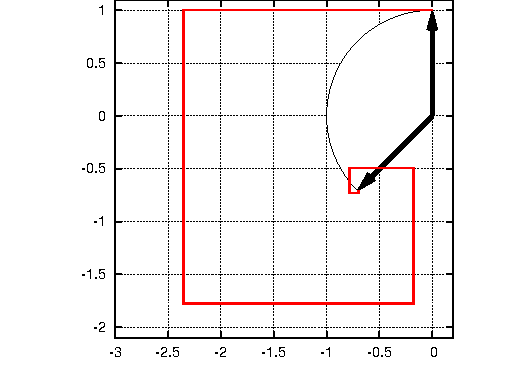
\epsfig{file=picts/C++/rotop-ulitka}
\end{center}
\caption{Пример поворота вектора $(0,1,0)$ на угол $3\pi/4$}\label{rotop:ulitka:pict} 
\end{figure}

\begin{figure}[p]
\begin{center}
\raisebox{1cm}{({\it а})}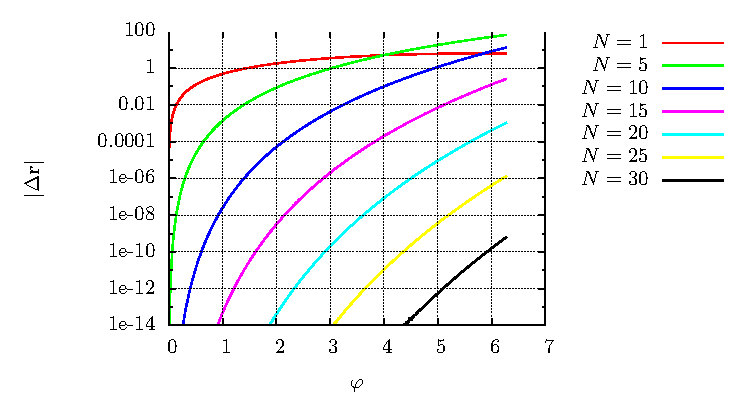
\epsfig{file=picts/C++/rotop-N-dR}
\vspace{-.5cm} 
\begin{tabular}{rl}
\raisebox{1cm}{({\it б})}\hspace{-1cm}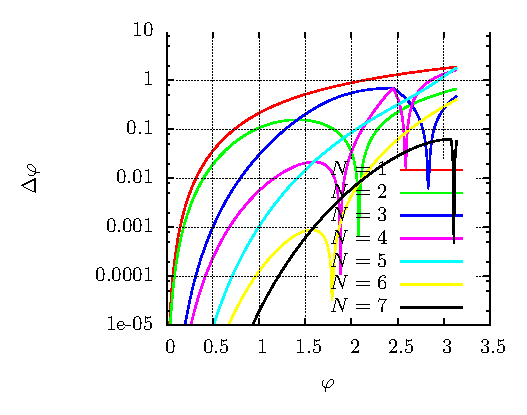
\epsfig{file=picts/C++/rotop-N-dphi} & \raisebox{1cm}{({\it в})}\hspace{-1cm}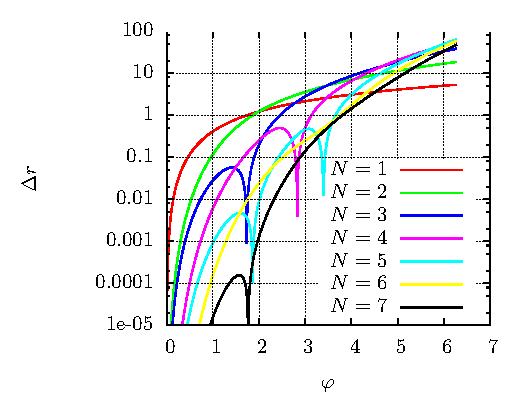
\epsfig{file=picts/C++/rotop-N-dr}\\[-.5cm]
\raisebox{1cm}{({\it г})}\hspace{-1cm}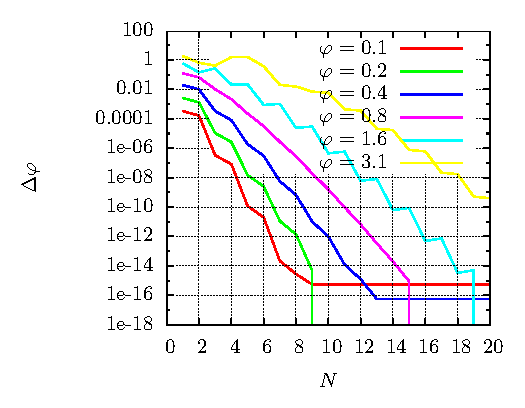
\epsfig{file=picts/C++/rotop-phi-dphi} & \raisebox{1cm}{({\it д})}\hspace{-1cm}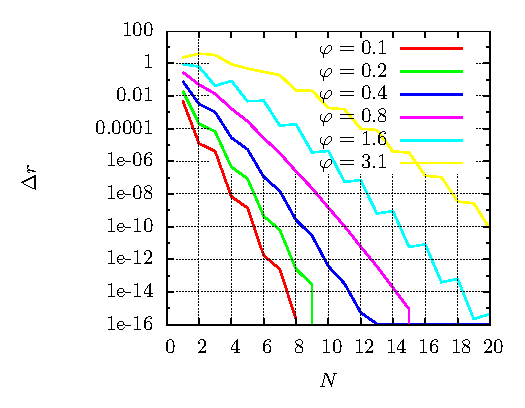
\epsfig{file=picts/C++/rotop-phi-dr}
\end{tabular}
\vspace{-.5cm} 
\end{center}
\caption{
Зависимости модуля ошибки $\vec r$ от угла поворота $\varphi$ единичного вектора $(0,1,0)$ для 
различного числа членов разложения~$N$ ({\it а}). Зависимости абсолютной ошибки по углу $\Delta\varphi$ ({\it б}) 
и модулю радиуса $\Delta r$ ({\it в}) от угла поворота $\varphi$
при использовании конечного числа членов разложения~$N$.  
Зависимости абсолютной ошибки по углу $\Delta\varphi$ ({\it г}) и радиусу $\Delta n$ ({\it д}) от числа членов разложения~$N$ 
для различных углов поворота~$\varphi$ }\label{rotop:delta:pict}
\end{figure}


Не теряя общности рассуждений, рассмотрим поворот вектора $(0,r_y,r_z)$ вокруг вертикальной оси на угол $\alpha$, 
и разложим  $\sin\alpha$ и $\cos\alpha$ в ряд в окрестностях точки $\alpha=0$:
$$
\vctr3{0}{r_y}{r_z}\rotop\vctr3{0}{0}{\alpha} = 
\vctr3{-r_y\sin\alpha}{r_y\cos\alpha}{r_z} = 
\vctr3{- r_y \sum\limits_{n=0}^\infty \frac{(-1)^n}{(2n+1)!} \alpha^{2n+1} }{
r_y\sum\limits_{n=0}^\infty \frac{(-1)^n}{(2n)!} \alpha^{2n} }{r_z} = 
\vctr3{- r_y \sum\limits_{n=0}^\infty \frac1{n!} \alpha^n \sin\frac{\pi n}2 }{
r_y\sum\limits_{n=0}^\infty \frac1{n!} \alpha^n \cos\frac{\pi n}2 }{r_z}. $$
Пусть $\a\times^n\b \equiv [...[\a \underbrace{\times \b]\times ... \b]}_n$ и $\a\times^0\b \equiv\a$. 
Рассмотрим последовательность векторных произведений:
\begin{align}
\vctr3{0}{r_y}{r_z}& \times\vctr3{0}{0}{\alpha} = \vctr3{\alpha r_y}{0}{0}, \quad 
\vctr3{0}{r_y}{r_z}\times^2\vctr3{0}{0}{\alpha} = \vctr3{0}{-\alpha^2 r_y}{0}, \quad 
\vctr3{0}{r_y}{r_z}\times^3\vctr3{0}{0}{\alpha} = \vctr3{-\alpha^3 r_y}{0}{0},  \notag\\
\vctr3{0}{r_y}{r_z}& \times^4\vctr3{0}{0}{\alpha} = \vctr3{0}{\alpha^4 r_y}{0}, \quad  ..., \quad
\vctr3{0}{r_y}{r_z}\times^n\vctr3{0}{0}{\alpha} = \vctr3{ \alpha^n r_y \sin\frac{\pi n}2}{\alpha^n r_y \cos\frac{\pi n}2}{0}.
\notag
\end{align}
Тогда, с учетом четности $\cos\alpha$ и нечетности $\sin\alpha$, поворот можно представить как
$$
\a \rotop \b = \sum\limits_{n=0}^\infty \frac1{n!}\a \times^n(-\b) = \sum\limits_{n=0}^\infty \frac{(-1)^n}{n!}\a \times^n\b.
$$


Этот же результат можно получить другим способом. Рассмотрим уравнение вида
\begin{equation}
\dot\a = -\left[ \a \times \vctr3{0}{0}{\omega} \right] \label{rotop:a:omega:eq}
\end{equation}
описывающее очевидно вращение вектора $\a$ вокруг вертикальной оси с угловой скоростью~$\omega$ против часовой стрелки (если смотреть сверху). 
Дифференцируя обе части уравнения (\ref{rotop:a:omega:eq}) по времени получаем рекуррентное соотношение для произвольной производной вектора $\a$ по времени:
$$
\frac{\partial^n\a}{\partial t^n} = -\left[ \frac{\partial^{n-1}\a}{\partial t^{n-1}} \times \vctr3{0}{0}{\omega} \right] = ... 
= (-1)^n \left[ \a \times^n \vctr3{0}{0}{\omega} \right].
$$
Пусть начальное значение вектора $\a|_{t=0}=\a_0$, тогда
$$
\a_0 \rotop \vctr3{0}{0}{\omega t} = \a(t).
$$
Разложим вектор $\a$ в ряд Тейлора в окрестности точки $t=0$:
$$
\a_0 \rotop \vctr3{0}{0}{\omega t} = \sum\limits_{n=0}^\infty \frac{t^n}{n!}\frac{\partial^n\a}{\partial t^n} = 
\sum\limits_{n=0}^\infty \frac{(-1)^n}{n!} \left[ \a \times^n \vctr3{0}{0}{\omega t} \right].
$$
Пример поворота на угол $3\pi/4$ приведен на рис.~\ref{rotop:ulitka:pict}.
Зависимости ошибок разложения приведены на рис.~\ref{rotop:delta:pict}.

Разложение оператора поворота в ряд может существенно ускорить численные схемы, использующие подобные конструкции. Так, поворот через матрицу 
(функция \verb'rotate' из модуля \verb'derart' библиотеки \verb'aivlib') занимает на процессоре {\sf Intel(R) Core(TM)2 CPU U7500} около 170 тактов,
а поворот через ряд (параметризованная по числу членов  разложения $R$ функция \verb'rotop<R>' из того же модуля) требует примерно 10 тактов 
на каждый из членов разложения.

Поскольку 
$$
\a\times^{n+2}\b = - b^2 \a\times^n\b 
$$
можно представить оператор поворота в виде суммы трех векторов
\begin{multline}
\a\rotop\b = \sum\limits_{n=0}^\infty \frac{(-1)^n}{n!} \a\times^n\b = 
\a - [\a\times\b] \sum\limits_{n=0}^\infty\frac{(-1)^n b^{2n}}{(2n+1)!} 
+\\+
\big[[\a\times\b]\times\b\big] \sum\limits_{n=0}^\infty\frac{(-1)^n b^{2n}}{(2n+2)!} 
\equiv
\a - [\a\times\b]\,\beta_1(b) - \big[\b\times[\a\times\b]\big]\, \beta_2(b)
=\\= 
\a\big(1-b^2\beta_2(b)\big) - [\a\times\b]\,\beta_1(b) + \b\,(\a\cdot\b)\,\beta_2(b),
\label{rotop:3v:rotop}
\end{multline}
где
$$
\beta_1(b) = \sum\limits_{n=0}^\infty\frac{(-1)^n b^{2n}}{(2n+1)!} = \frac{\sin b}b ,
\qquad
\beta_2(b) = \sum\limits_{n=0}^\infty\frac{(-1)^n b^{2n}}{(2n+2)!} = \frac{1-\cos b}{b^2},
$$
или
$$
\a\rotop\b = \a \cos b - [\a\times\n_b] \sin b + \n_b (\a \cdot \n_b)(1-\cos b).
$$


%\subsection{Дифференцирование оператора поворота}
Рассмотрим выражение $\partial(\a\rotop\varphi\b)/\partial\varphi$, где $\b$~вектор задающий ось вращения.
\begin{multline}
\dfdx{(\a\rotop\varphi\b)} \varphi = \dfdx{}{\varphi}
\sum\limits_{n=0}^\infty \frac{(-1)^n}{n!} \a \times^n \varphi\b = 
\sum\limits_{n=1}^\infty \frac{(-1)^n\varphi^{n-1}}{(n-1)!} \a \times^n \b = \\ =
-\left[\sum\limits_{n=1}^\infty \frac{(-1)^{n-1}}{(n-1)!} \a \times^n\varphi\b\right]\times\b = 
-(\a\rotop\varphi\b)\times\b = \b \times(\a\rotop\varphi\b).
\notag%\label{diff:rotop:eq}
\end{multline}

\endinput
%%%%%%%%%%%%%%%%%%%%%%%%%%%%%%%%%%%%%%%%%%%%%%%%%%%%%%%%%%%%%
%Аналогично, 
Рассмотрим выражение $\partial(\a(t)\rotop\varphi(t)\b)/\partial t$, где $\b$~вектор задающий ось вращения:
\begin{multline}
\dfdx{(\a(t)\rotop\varphi(t)\b)} t = \dfdx{}{t}
\sum\limits_{n=0}^\infty \frac{(-1)^n}{n!} \a(t) \times^n \varphi(t)\b = \\
= \sum\limits_{n=0}^\infty \frac{(-1)^n}{n!}\left[ \dfdx\a t \times^n \varphi \b +
 n \varphi^{n-1} \dfdx\varphi t \a \times^n \b \right] = \\ =
\dfdx\a t \rotop \varphi \b -\dfdx\varphi t \left[\sum\limits_{n=1}^\infty \frac{(-1)^{n-1}}{(n-1)!} \a \times^{n-1}\varphi\b\right]\times\b = \\
 = \dfdx\a t \rotop \varphi \b + \dfdx\varphi t \b \times(\a\rotop\varphi\b).
\label{rotop:da:dt:eq}
\end{multline}

На основе (\ref{rotop:3v:rotop}) получаем
$$
\beta_1'(b) = \frac{b\cos b-\sin b}{b^2}, \qquad \beta_2'(b) = \frac{b^2 \sin b - 2b(1-\cos b)}{b^4},
$$
откуда
\begin{multline}
\dfdx{(\a(t)\rotop\b(t))} t = 
\dot\a\big(1-b^2\beta_2(b)\big) - \a\big(2b\beta_2(b)\dot b + b^2\beta'_2(b)\dot b\big) 
-\\- [\dot\a\times\b]\,\beta_1(b) - [\a\times\dot\b]\,\beta_1(b) - [\a\times\b]\,\beta'_1(b) \dot b
+\\+ \dot\b\,(\a\cdot\b)\,\beta_2(b) + \b\,(\dot\a\cdot\b)\,\beta_2(b) + \b\,(\a\cdot\dot\b)\,\beta_2(b) +
\b\,(\a\cdot\b)\,\beta_2'(b) \dot b
=\\=
\dot\a \cos b + \a \dot b \sin b
- [\dot\a\times\b]\,\beta_1(b) - [\a\times\dot\b]\,\beta_1(b) - [\a\times\b]\,\frac{b\cos b-\sin b}{b^2} \dot b
+\\+ \dot\b\,(\a\cdot\b)\,\beta_2(b) + \b\,(\dot\a\cdot\b)\,\beta_2(b) + \b\,(\a\cdot\dot\b)\,\beta_2(b) +
\b\,(\a\cdot\b)\,\frac{b^2 \sin b - 2b(1-\cos b)}{b^4} \dot b
.
\label{rotop:da:dt:33v:eq}
\end{multline}

\begin{multline}
\dfdx{\a\rotop\b} t = \dot\a \cos b - \a\dot b \sin b 
- [\dot\a\times\n_b] \sin b - [\a\times\dot\n_b] \sin b  - [\a\times\n_b] \dot b\cos b 
+\\+ \dot\n_b (\a \cdot \n_b)(1-\cos b) + \n_b (\dot\a \cdot \n_b)(1-\cos b) + \n_b (\a \cdot \dot\n_b)(1-\cos b) 
+ \n_b (\a \cdot \n_b)\dot b \sin b 
=\\=
\dot\a \cos b - [\dot\a\times\n_b] \sin b + \n_b (\dot\a \cdot \n_b)(1-\cos b)  
-\\- 
\a\dot b \sin b - [\a\times\n_b] \dot b\cos b + \n_b (\a \cdot \n_b)\dot b \sin b 
-\\- [\a\times\dot\n_b] \sin b   
+ \dot\n_b (\a \cdot \n_b)(1-\cos b)  + \n_b (\a \cdot \dot\n_b)(1-\cos b) 
\end{multline}






